\documentclass{hbrs-ecta-report}

\usepackage{float}
\usepackage{placeins}
\usepackage{ngerman}
\usepackage[utf8]{inputenc}
\begin{document}

\conferenceinfo{H-BRS}{2017}

\title{Neuroevolution: Simple Genetic Algorithm}
\subtitle{}

\numberofauthors{2}
\author{
\alignauthor
Tim L"ugger, Jan Urfei
}

\date{today}
\maketitle
\begin{abstract}
Aufgabe: Implementiere einen Genetische Algorithmus und führe diesen 100 mal mit einer vorgegebenen Kostenfunktion aus. Ziel ist es das Minimum der Egg Funktion zu finden.
\end{abstract}

\section{Der Genetische Algorithmus}
Der Genetische Algorithmus besitzt eine Population, welches eine Menge fester Größe an verschiedenen Lösungen ist. Diese Population wird pro Durchlauf verändert. Einen Durchlauf nennt man eine Generation. 
\newline \newline
Als erstes wählt man ''zufällig'' Elternpaare für die nächste Generation aus. Für diese Auswahl gibt es verschiedene Verfahren auf die wir hier nicht näher eingehen. Diese Elternpaare werden verglichen und der Teil der den besseren Fitnesswert hat kommt in die neue Population der nächsten Generation. Der Beste (die Elite) der alten Generation wird einfach übernommen.
\newline \newline
Danach werden aus der neu gebildeten Menge zu einer gewissen Wahrscheinlichkeit  2 Lösungen genommen, die zueinander vereint werden und eine neue Lösung bilden. Diesen Vorgang nennt man Crossover.
\newline \newline
Nachdem Crossover nimmt man sich noch einen gewissen Prozentsatz aller Lösungen und mutiert diese, d.h. diese werden minimal zufällig verändert, sodass eine neue ähnliche Lösung entsteht.
\newline \newline
Jetzt  hat sich eine neue Population gebildet, die die alte beste Lösung beinhaltet und neue ähnliche Lösungen, um vielleicht noch bessere zu finden. Die Populationsgröße, der Wahrscheinlichkeit zum mutieren und für den Crossover, sowie die Anzahl an Generationen sind Parameter, die das Ergebnis sehr stark beeinflussen können.

\FloatBarrier

\section{Herangehensweise}
Die Anfangspopulation wird zufällig aus Koordinatenpaaren gebildet, die innerhalb des gültigen Wertebereichs [-512 ; 512] liegen. Von allen Lösungen berechnen wir danach die Fitness. Als Kostenfunktion nutzen wir die Egg Funktion (Figure \ref{fig:egg}). 

\begin{figure}[h]
	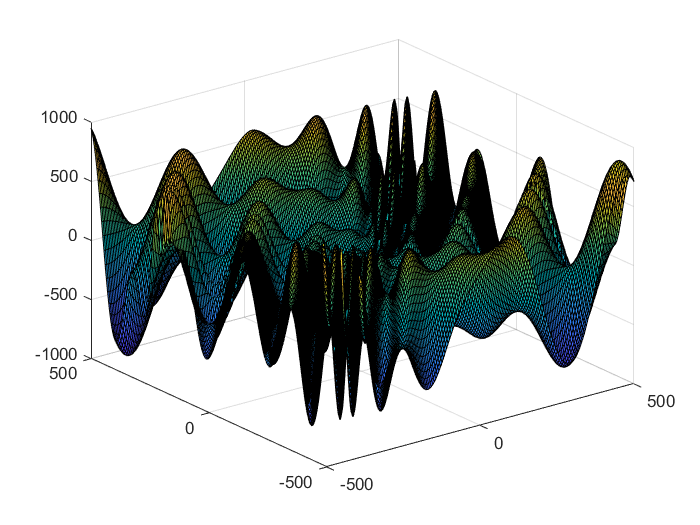
\includegraphics[width=\linewidth]{img/egg}
	\caption{3D Eggholder function: defined between -512 and 512}
	\label{fig:egg}
\end{figure}

Das Genom mit dem besten Ergebnis (dem niedrigsten egg(Genom)) wird unverändert in die neue Population übernommen.
Mit der restlichen Population wird eine Tournament Selection durchgeführt. Dazu wird für jedes zu erzeugende Kind jeweils 2 Genome zufällig  ausgewählt und das mit der höheren Fitness übernommen. \newline
Nun wird mit einer bei diesen Kindergenomen mit einer gewissen Wahrscheinlichkeit die x bzw. y Werte untereinander vertauscht (Crossover).
\newline
Anschließend werden die meisten (mutationRate) der Kindergenome noch mutiert. Es werden die x und y Werte jeweils mit einer zufällig, normal verteilten Zahl addiert. (Mutation)

\FloatBarrier
\newpage

\section{Unsere Ergebnisse}

Es wurden 100 Genome für die Populationen verwendet sowie 100 Experimente mit je 100 Iterationen durchgeführt.

Man erkennt in Figure \ref{fig:fitness} das die Werte der Kostenfunktion innerhalb der ersten ~20 Iterationen stark fällt und dann in Werten um -900 Konvergiert. Zu beachten ist auch, dass allein in der Startpopulation, die Elite schon nah am niedrigsten Wert ist. \newline
Als minimalen Werten konnten wird egg([522.1469,413.3025]) = -976.9110 ausmachen. Da dies aber der Angabe vom Globalen Minimum von -959.6407 widerspricht wird vermutet, dass es sich um eine Ungenauigkeit bei der Fließkommaberechnung handelt.

An Figure \ref{fig:elite} lässt sich gut erkennen, welchen Einfluss der Nichtdeterminismus des Algorithmus auf das Finden eines Minimums. Denn nur in wenigen Experimenten wurden Minima $\leq -950$ gefunden. Teilweise sogar auch nur Werte $\ge -800$.
\begin{figure}[h]
	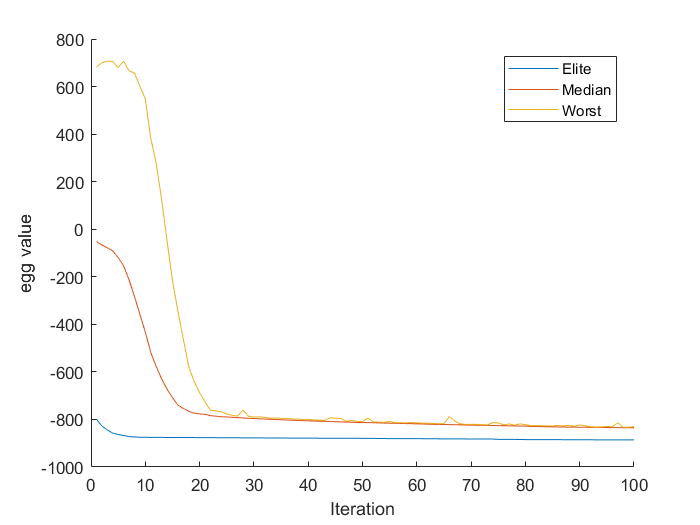
\includegraphics[width=\linewidth]{img/fitness-history}
	\caption{Fitness during iterations with mean over all experiments}
	\label{fig:fitness}
\end{figure}
\begin{figure}[h]
	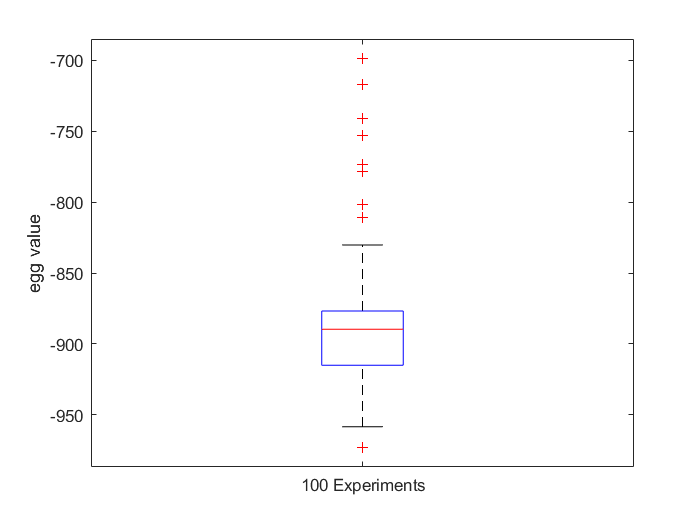
\includegraphics[width=\linewidth]{img/elite-range-boxplot}
	\caption{Elite fitness in last iteration step of every experiment}
	\label{fig:elite}
\end{figure}


\end{document}
}